\subsection{Delta Squared-DFT}
{{\footnotesize
\noindent Introduces the Delta Squared-ML paradigm-using ML corrections to DFT to predict reaction energies with accuracy comparable to CCSD(T), while training on small CC datasets. Evaluated across 10 reaction datasets covering organic and organometallic transformations.


\begin{description}[labelwidth=4cm, labelsep=1em, leftmargin=4cm, itemsep=0.1em, parsep=0em]
  \item[date:] 2024-12-13
  \item[version:] v1.0
  \item[last\_updated:] 2024-12
  \item[expired:] unknown
  \item[valid:] yes
  \item[valid\_date:] 2024-12-13
  \item[url:] \href{https://neurips.cc/virtual/2024/poster/97788}{https://neurips.cc/virtual/2024/poster/97788}
  \item[doi:] 10.48550/arXiv.2406.14347
  \item[domain:] Computational Chemistry; Materials Science
  \item[focus:] Benchmarking machine-learning corrections to DFT using Delta Squared-trained models for reaction energies
  \item[keywords:]
    - density functional theory
    - Delta Squared-ML correction
    - reaction energetics
    - quantum chemistry
  \item[licensing:] unknown
  \item[task\_types:]
    - Regression
  \item[ai\_capability\_measured:]
    - High-accuracy energy prediction
    - DFT correction
  \item[metrics:]
    - Mean Absolute Error (eV)
    - Energy ranking accuracy
  \item[models:]
    - Delta Squared-ML correction networks
    - Kernel ridge regression
  \item[ml\_motif:]
    - Scientific ML
  \item[type:] Dataset + Benchmark
  \item[ml\_task:]
    - Regression
  \item[solutions:] Solution details are described in the referenced paper or repository.
  \item[notes:] Demonstrates CC-level accuracy with \textasciitilde{}1\% of high-level data. Benchmarks publicly included for reproducibility.

  \item[contact.name:] Wei Liu
  \item[contact.email:] unknown
  \item[results.links.name:] ChatGPT LLM
  \item[fair.reproducible:] Yes
  \item[fair.benchmark\_ready:] Yes
  \item[id:] delta\_squared-dft
  \item[Citations:] \cite{khrabrov2024nabla2dftuniversalquantumchemistry}
\end{description}

{\bf Ratings:} ~ \\

\begin{tabular}{p{0.15\textwidth} p{0.07\textwidth} p{0.7\textwidth}}
\hline
Rating & Value & Reason \\
\hline
dataset & 4.5 & Multi-modal quantum chemistry datasets are standardized and accessible; repository available.
 \\
documentation & 4 & Source code supports pipeline reuse, but formal evaluation splits may vary.
 \\
metrics & 4 & Uses standard regression metrics like MAE and energy ranking accuracy; appropriate for task.
 \\
reference\_solution & 3.5 & Includes baseline regression and kernel ridge models; implementations are reproducible.
 \\
software & 3 & Source code and baseline models available for ML correction to DFT; framework maturity is moderate.
 \\
specification & 4 & Benchmark focuses on reaction energy prediction with clear goals, though some task specifics could be formalized further.
 \\
\hline
\end{tabular}

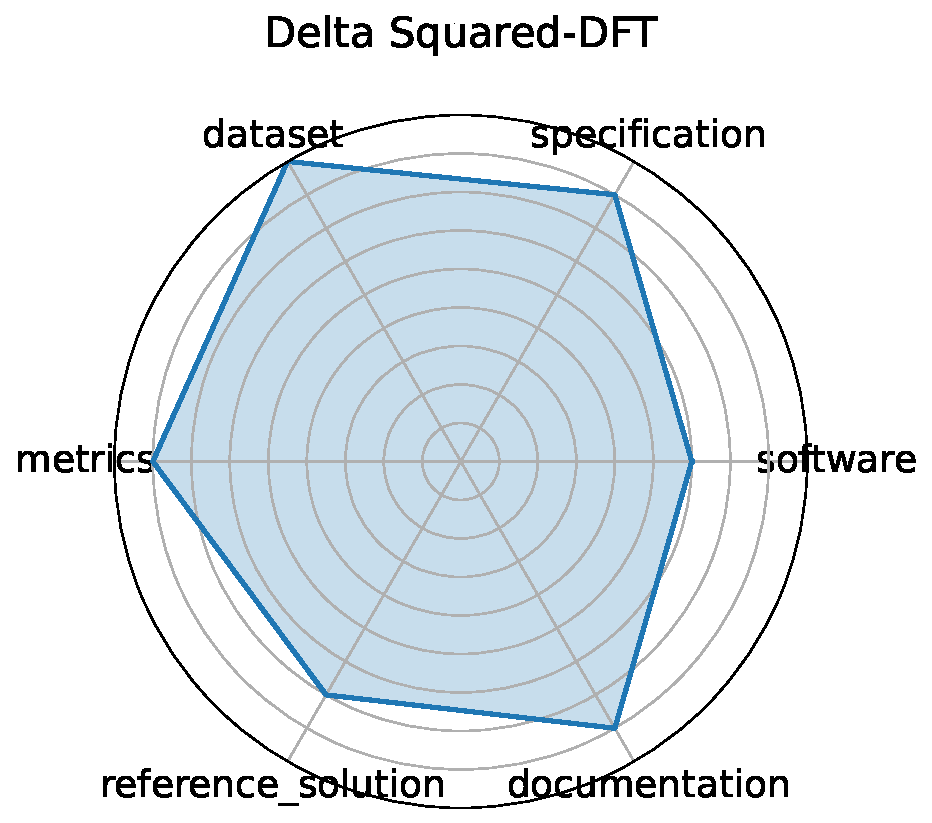
\includegraphics[width=0.2\textwidth]{delta_squared-dft_radar.pdf}
}}
\clearpage